\section{Things and Stuff}
\begin{frame}{}
    \LARGE Image Segmentation: \textbf{Things and Stuff}
\end{frame}

\begin{frame}{Things and Stuff}
\begin{columns}
    \begin{column}{0.5\textwidth}
        \begin{itemize}
            \item \textbf{Things:} Object categories that can be separated into object instances (e.g. cats, cars, person)
            \item \textbf{Stuff:} Object categories that cannot be separated into instances (e.g. sky, grass, water, trees)
        \end{itemize}
    \end{column}
    \begin{column}{0.5\textwidth}
        \begin{figure}
        \centering
        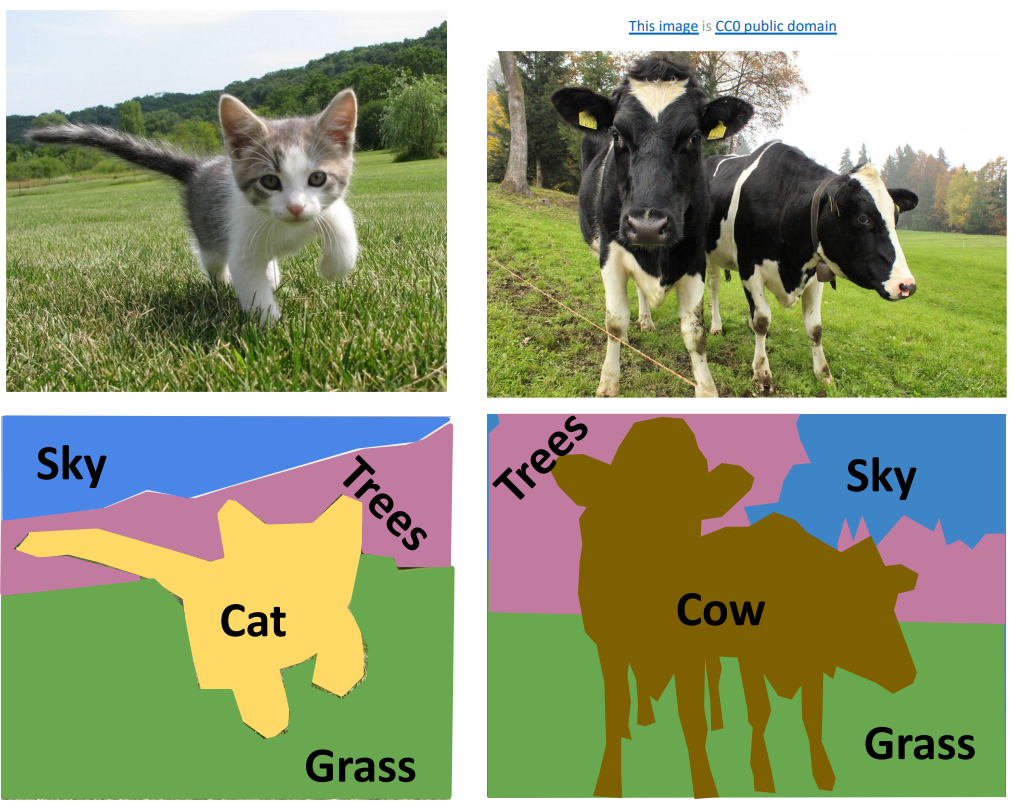
\includegraphics[width=1.0\textwidth,height=1.0\textheight,keepaspectratio]{images/segmentation/ins_1.png}
        \end{figure}
    \end{column}
\end{columns}
    
\end{frame}

\begin{frame}{Computer Vision Tasks}
\begin{columns}
    \begin{column}{0.5\textwidth}
        \begin{itemize}
            \item \textbf{Object Detection:} Detects individual object instances, but only gives box(Only things!)
        \end{itemize}
        \begin{figure}
        \centering
        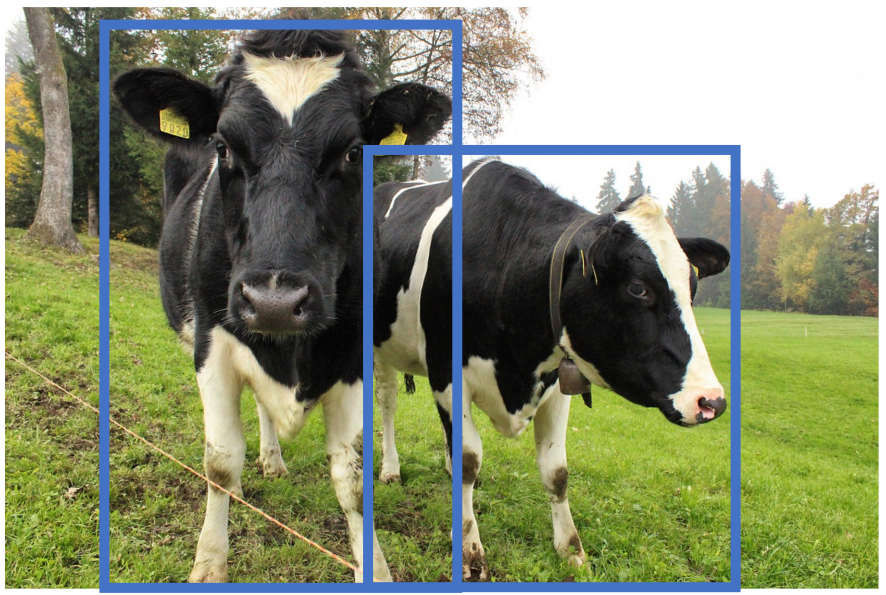
\includegraphics[width=1.0\textwidth,height=1.0\textheight,keepaspectratio]{images/segmentation/ins_2.png}
        \end{figure}
    \end{column}
    \begin{column}{0.5\textwidth}
        \begin{itemize}
            \item \textbf{Semantic Segmentation:} Gives per-pixel labels, but merges instances (Both things and stuff)
        \end{itemize}
        \begin{figure}
        \centering
        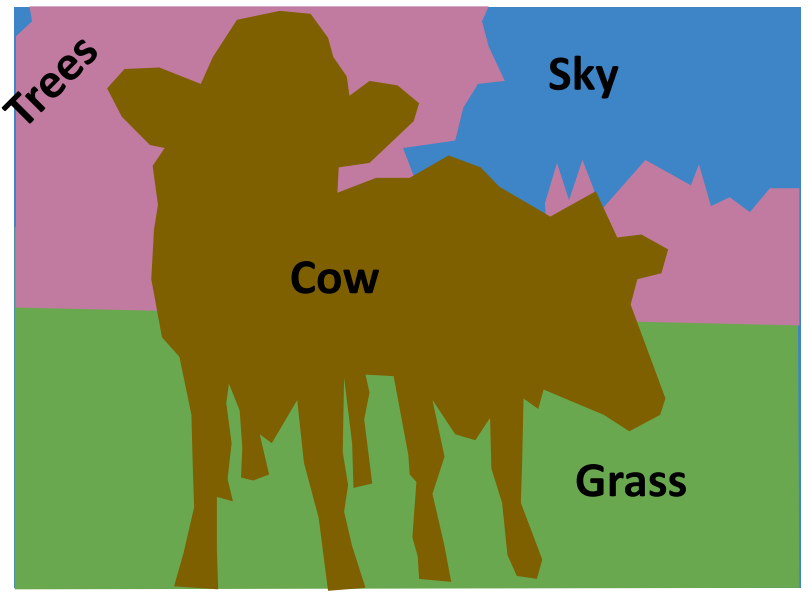
\includegraphics[width=1.0\textwidth,height=1.0\textheight,keepaspectratio]{images/segmentation/ins_3.png}
        \end{figure}
    \end{column}
\end{columns}
    
\end{frame}